\documentclass[a4paper,12pt]{article} % Тип документа



\usepackage{graphicx}
\graphicspath{{pictures/}}
\DeclareGraphicsExtensions{.pdf,.png,.jpg}
\usepackage{multirow}

% Русский язык
\usepackage[T2A]{fontenc}
\usepackage[utf8]{inputenc}
\usepackage[english,russian]{babel}

% Математика
\usepackage{amsmath,amsfonts,amssymb,amsthm,mathtools} 


\usepackage{wasysym}

%Заговолок
\author{Маллаев Руслан}
\title{Лабораторная работа №1.2.2}
\date{25 октября 2020 г.}

\begin{document} % Начало документа

\maketitle
\newpage
 
 \textbf{Цель работы:}  экспериментально проверить уравнение вращатель-
 
 ного движения, получив зависимость углового ускорения от момента
 
 инерции и момента 
прикладываемых к системе сил, а также проана-

лизировать влияние сил трения, действующих в оси вращения.
\\

\textbf{Приборы, используемые в работе:} маятник обербека, разновесы,

штангенциркуль, компьютер с предустановленной программой, дат-

чик движения.\\


Соберем установку, как показано на рисунке 1:
\[\text{Рисунок №1}\]
\begin{center}
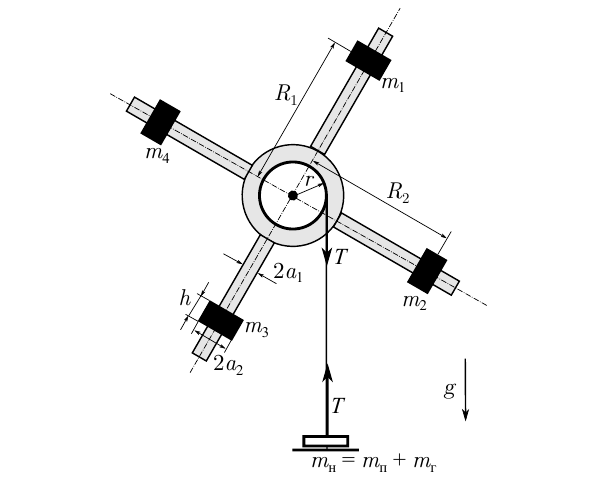
\includegraphics[scale=0.89]{обербексхема}
\end{center}

\newpage
\section{Балансировка}
$l_1 = (2.496\pm0.001)\text{см};\text{ }l_2 = (2.500\pm0.001)\text{см};\text{ }l_3 = (2.500\pm0.001)\text{см};\text{ }l_4 = (2.500\pm0.001)\text{см}$, где l - длина грузов.\\\\
Тогда $R_1 - \frac{l_1}{2} = (8,040\pm0.001)\text{см};\text{ }R_2 - \frac{l_2}{2} = (8,110\pm0.001)\text{см};\text{ }R_3 - \frac{l_3}{2} = (8,650\pm0.001)\text{см};\text{ }R_4 - \frac{l_4}{2} = (8,260\pm0.001)\text{см};\text{ }$

\[R_1 = (9.288\pm0.002)\text{см}\]
\[R_2 = (9.360\pm0.002)\text{см}\]
\[R_3 = (9.900\pm0.002)\text{см}\]
\[R_4 = (9.510\pm0.002)\text{см}\]

\[2r_{\text{бш}}(\text{радиус большого шкива}) = (3.510\pm0.001)\text{см}\]
\[2r_{\text{мш}}(\text{радиус малого шкива}) = (1.800\pm0.001)\text{см}\]



\section{Оценка момента сил трения покоя $M_0$}
Масса платформы $m_{\text{п}} = 6.171\text{г}$ при подвешивании платформы на малый шкив маятник медленно начинает вращаться, значит
\[M_0 < m_{\text{п}}\cdot g\cdot r_{\text{мш}} = 11 \cdot 10^{-3} \text{Н}\]
То есть точно измерить его у нас не получится



\section{Измерение коэффициентов прямой $\beta = \beta_0 + k\omega$ и обработка результатов измерения}
\begin{itemize}
\item $m_{\text{г}} = (30.1\pm0.1)\text{г}$, большой шкив\\
1)$\beta_0 = (0.5267\pm0.0330)\frac{\text{рад}}{\text{с}^2}$\\
$\text{ }\text{ }$ $k = (-0.02036\pm0.02700)\frac{1}{\text{с}}$

2)$\beta_0 = (0.5769\pm0.0086)\frac{\text{рад}}{\text{с}^2}$\\
$\text{ }\text{ }$ $k = (-0.02377\pm0.00670)\frac{1}{\text{с}}$

3)$\beta_0 = (0.5470\pm0.0089)\frac{\text{рад}}{\text{с}^2}$\\
$\text{ }\text{ }$ $k = (-0.02227\pm0.00730)\frac{1}{\text{с}}$

4)$\beta_0 = (0.5793\pm0.0090)\frac{\text{рад}}{\text{с}^2}$\\
$\text{ }\text{ }$ $k = (-0.02522\pm0.00710)\frac{1}{\text{с}}$

5)$\beta_0 = (0.5917\pm0.0078)\frac{\text{рад}}{\text{с}^2}$\\
$\text{ }\text{ }$ $k = (-0.02916\pm0.00660)\frac{1}{\text{с}}$

\[\sigma_{\beta} = \frac{1}{N}\cdot\sqrt{\sum_{i = 1}^{n}(\overline{\beta}-\beta_i)^2}\]
\[\sigma_{\beta} = 0.0107\frac{\text{рад}}{\text{с}^2}\text{ -- случайная погрешность}\]
\[M_1 = 1.25\cdot10^{-2}H\cdot\text{м}\]
\item $m_{\text{г}} = (62.9\pm0.1)\text{г}$, большой шкив\\
$\beta_0 = (0.5917\pm0.0078)\frac{\text{рад}}{\text{с}^2}$\\
$k = (-0.02916\pm0.00660)\frac{1}{\text{с}}$
\[M_2 = 1.29\cdot10^{-2}H\cdot\text{м}\]
\item $m_{\text{г}} = (93.0\pm0.1)\text{г}$, большой шкив\\
$\beta_0 = (1.2000\pm0.0015)\frac{\text{рад}}{\text{с}^2}$\\
$k = (-0.01481\pm0.00078)\frac{1}{\text{с}}$
\[M_3 = 1.77\cdot10^{-2}H\cdot\text{м}\]
\item $m_{\text{г}} = (127.1\pm0.1)\text{г}$, большой шкив\\
$\beta_0 = (1.7140\pm0.0099)\frac{\text{рад}}{\text{с}^2}$\\
$k = (-0.02406\pm0.00430)\frac{1}{\text{с}}$
\[M_4 = 2.32\cdot10^{-2}H\cdot\text{м}\]
\item $m_{\text{г}} = (62.9\pm0.1)\text{г}$, малый шкив\\
$\beta_0 = (0.5027\pm0.0080)\frac{\text{рад}}{\text{с}^2}$\\
$k = (-0.02283\pm0.00520)\frac{1}{\text{с}}$
\[M_5 = 0.57\cdot10^{-2}H\cdot\text{м}\]
\item $m_{\text{г}} = (93.0\pm0.1)\text{г}$, малый шкив\\
$\beta_0 = (0.6187\pm0.0056)\frac{\text{рад}}{\text{с}^2}$\\
$k = (-0.01684\pm0.00270)\frac{1}{\text{с}}$
\[M_6 = 0.79\cdot10^{-2}H\cdot\text{м}\]
\item $m_{\text{г}} = (127.1\pm0.1)\text{г}$, малый шкив\\
$\beta_0 = (0.9422\pm0.0940)\frac{\text{рад}}{\text{с}^2}$\\
$k = (-0.02827\pm0.03700)\frac{1}{\text{с}}$
\[M_7 = 1.03\cdot10^{-2}H\cdot\text{м}\]
\end{itemize}
Построим графики зависимости $\beta_0$ от $M$ для малого и большого шкивов на графике №1:
\begin{center}
\[\text{График №1}\]
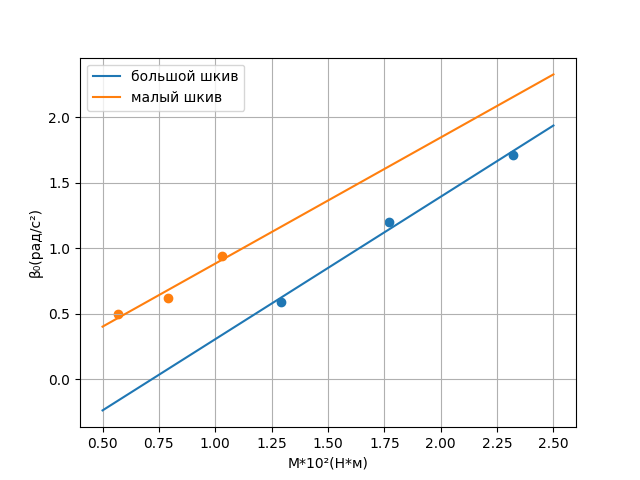
\includegraphics[scale=0.8]{graphoberi}
\end{center}
Откуда найдем значения моментов инерции как величину обратную к коэффициенту наклона графиков:
\[I_{\text{м}} = 10.4\cdot10^{-3}\text{кг}\cdot\text{м}^2\]
\[I_{\text{б}} = 9.2\cdot10^{-3}\text{кг}\cdot\text{м}^2\] 
Значения немного отличаются, это можно объяснить малым количеством точек и разбалансировкой
\[\overline{I} = 9.8\cdot10^{-3}\text{кг}\cdot\text{м}^2\]




\section{Измерение зависимости углового ускорения от момента инерции системы}
\[I = \frac{m_{\text{н}}\cdot g\cdot R}{\beta_0}\]
Измерения будут проводиться для $m_{\text{г}} = 100\text{г}$; Результаты измерений занесем в таблицу №1:
\[\text{Таблица №1}\]
\begin{center}
\begin{tabular}{|c|c|c|c|}
\hline
R, см & 10.73        & 11.83        & 13.06        \\ \hline
$\beta_0,\frac{\text{рад}}{\text{с}^2}$     & 1.53±0.10    & 1.21±0.01    & 1.09±0.01    \\ \hline
k, $\frac{1}{\text{с}}$     & -0.040±0.047 & -0.018±0.004 & -0.017±0.004 \\ \hline
I$\cdot10^{3}$, Н$\cdot$м     & 12.4         & 15.7         & 17.4         \\ \hline
\end{tabular}
\end{center}
Построим график зависимости I от $R^2$ на графике №2, чтобы проверить формулу
\[I = \sum_i m_i\cdot R_i^2\]
\begin{center}
\[\text{График №2}\]
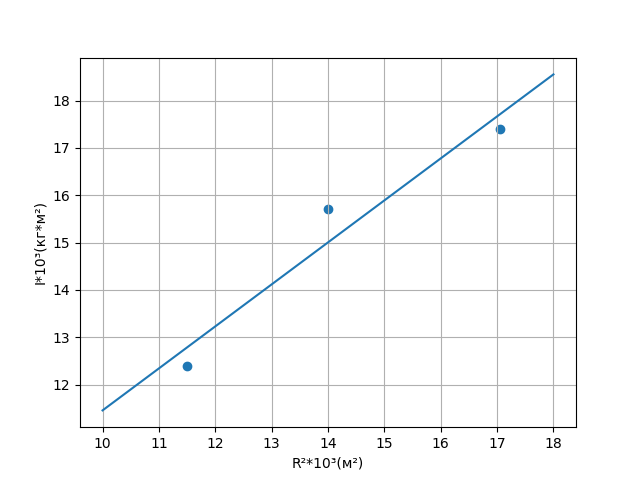
\includegraphics[scale=0.8]{graphi}
\end{center}
Из графика получим $I_0$, равный точке, в которой прямая пересекает ось y:
\[I_0 = 2.58\cdot10^{-3}\text{кг}\cdot\text{м}^2\]



\section{Измерение углового ускорения для маятника Обербека без грузов}
\[I_0 = \frac{m_{\text{н}}\cdot g\cdot R}{\beta_0}\]
\begin{itemize}
\item $m_{\text{г}} = (62.9\pm0.1)\text{г}$, большой шкив\\
$\beta_0 = (2.43\pm0.01)\frac{\text{рад}}{\text{с}^2}$\\
$k = (-0.0483\pm0.0026)\frac{1}{\text{с}}$
\[I_0 = 5.21\cdot10^{-3}\text{кг}\cdot\text{м}^2\]
\item $m_{\text{г}} = (100.0\pm0.1)\text{г}$, большой шкив\\
$\beta_0 = (3.54\pm0.01)\frac{\text{рад}}{\text{с}^2}$\\
$k = (-0.0514\pm0.0034)\frac{1}{\text{с}}$
\[I_0 = 5.29\cdot10^{-3}\text{кг}\cdot\text{м}^2\]
\item $m_{\text{г}} = (144.6\pm0.1)\text{г}$, большой шкив\\
$\beta_0 = (5.01\pm0.11)\frac{\text{рад}}{\text{с}^2}$\\
$k = (-0.0684\pm0.0029)\frac{1}{\text{с}}$
\[I_0 = 5.17\cdot10^{-3}\text{кг}\cdot\text{м}^2\]
\[\Delta_{\overline{I_0}} = 0.54\cdot10^{-3}\text{кг}\cdot\text{м}^2\]
\[\overline{I_0} = 5.22\cdot10^{-3}\text{кг}\cdot\text{м}^2\]
\end{itemize}
\section{Вывод}
Мы на практике проверили закон вращательного движения и нашли свободный момент инерции маятника Обербека



\end{document}